\documentclass[helvetica, 10pt]{article}

% If you're new to LaTeX, here's some short tutorials:
% https://www.overleaf.com/learn/latex/Learn_LaTeX_in_30_minutes
% https://en.wikibooks.org/wiki/LaTeX/Basics

% Formatting
\usepackage{blindtext}
\usepackage[T1]{fontenc}
\usepackage[utf8]{inputenc}
\usepackage[margin=1in]{geometry}

% Math
% https://www.overleaf.com/learn/latex/Mathematical_expressions
\usepackage{amsmath, amsfonts, amssymb, mathtools}

% Images
% https://www.overleaf.com/learn/latex/Inserting_Images
\usepackage{graphicx, float}

% Algorithms
% https://www.overleaf.com/learn/latex/algorithms
% https://en.wikibooks.org/wiki/LaTeX/Algorithms
\usepackage[ruled,vlined]{algorithm2e}
\usepackage{algorithmic}

% Code syntax highlighting
% https://www.overleaf.com/learn/latex/Code_Highlighting_with_minted
\usepackage{minted}
\usemintedstyle{borland}


% ====================== TITLE =========================================
\title{Artificial intelligence - Project 2 \\ - Dominos and The Resistance - }

% introduceti numele autorului aici
\author{George Botis & Daria Francioli}
\date{10/12/2022}

\begin{document}

\maketitle
\thispagestyle{empty}

\section{Introducere}

Scopul acestui proiect este acela de a implementa:
\begin{enumerate}
    \item un program care rezolvă diferite lvl pentru faimosul joc de Domino.
    \item un program care încearcă să rezolve puzzle-ul deducerii rolurilor jucătorilor din jocul „The Resistance”.
\end{enumerate} 
\newline
\subsection{Domino}

Domino este un joc celebru cu piese de domino. Doi sau mai mulți jucători trebuie să pună alternativ piesele potrivite. Câștigătorul este persoana care scapă mai întâi de toate piesele sale.
\newline
\newline
\begin{figure}[h]
    \centering
    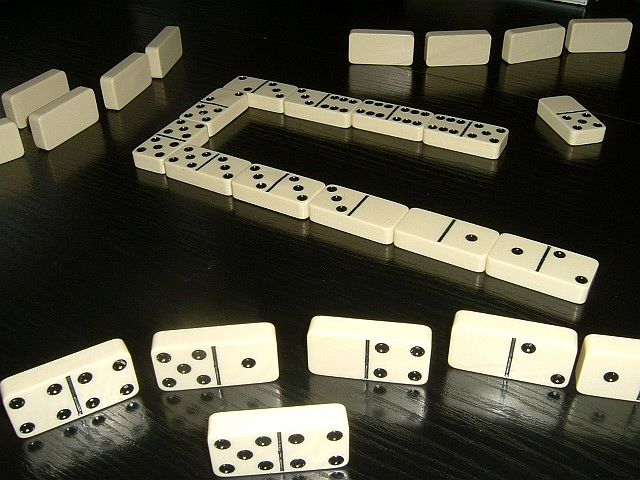
\includegraphics[width=16cm]{text/images/pic1.jpg}\\
    \caption{Domino}
\end{figure}

Avem nevoie de opt secvențe de șapte pătrate pentru piese. În total sunt 56 de pătrate. Ele reprezintă numerele de la 0 la 6. Numerele sunt reprezentate de puncte ca pe zarurile de joc. Un pătrat gol ia locul numărului 0.

\newpage
\subsection{The Resistance}

The Resistance este un joc de deducție socială care implică jucătorii care încearcă să-și dea seama cine dintre ei face parte din „Rezistență” și cine face parte din echipa „Guvernul”. Jocul este plasat într-o lume fictivă în care Rezistența încearcă să răstoarne un guvern tiranic, iar echipa de spionaj lucrează pentru a le sabota eforturile.
\newline
\newline
Fiecărui jucător i se atribuie în secret un rol la începutul jocului, iar scopul jocului este ca echipa Rezistenței să finalizeze cu succes o serie de misiuni fără a fi detectată de echipa de spionaj. Echipa de spionaj, pe de altă parte, vrea să împiedice Rezistența să reușească votând împotriva propunerilor de misiune și încercând să-și dea seama cine sunt ceilalți spioni.
\newline
\newline

\newline

\begin{figure}[h]
    \centering
    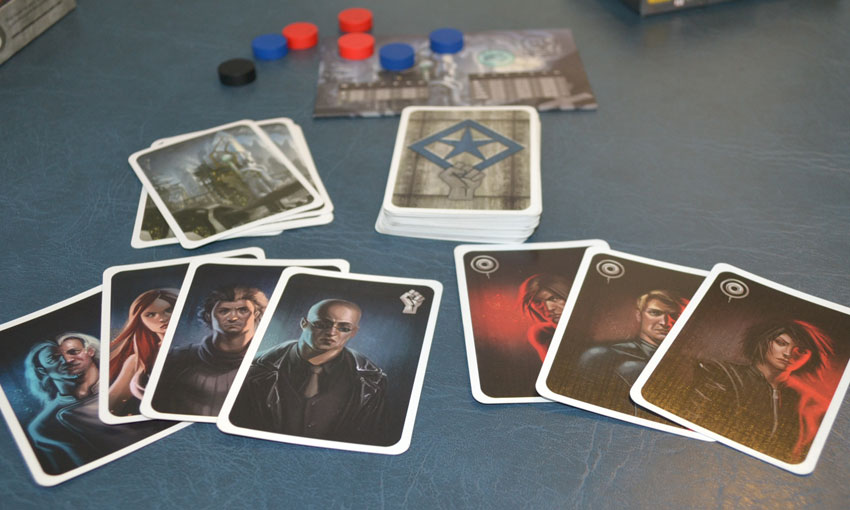
\includegraphics[width=16cm]{text/images/pic2.jpg}\\
    \caption{The Resistance Board Game}
\end{figure} \newline
\newline

\newline


\newline

\newline
Mai avem si jucători de tip Trădători, în echipa de spioni care lucrează în secret împotriva celorlalți din guvern. Acest jucător are propriile obiective secrete pe care trebuie să încerce să le ducă la bun sfârșit, încercând, de asemenea, să se îmbine cu ceilalți spioni.

Trădătorul este o răsturnare a jocului tradițional Resistance care adaugă un strat suplimentar de înșelăciune, intrigă și face și jocul mai complex.



\section{Definirea problemei}
% enuntul intrebarii
În această secțiune vom prezenta problma fiecărui puzzle.
\newline


\subsection{Domino - Seven Squares}

\begin{enumerate}
    \item Prima Problemă\newline\newline
 Așezarea a șapte cadre pătrate cu toate cele 28 de piese de domino. Dominourile cu același număr de puncte se întâlnesc.\newline
    \item A doua Problemă\newline\newline
Așezarea a șapte cadre pătrate cu toate cele 28 de piese de domino, astfel încât sumele numerelor de puncte să fie aceleași pe toate cele patru laturi. \newline
Suma este 4 + 4 + 2 = 2 + 2 + 6 = 6 + 1 + 3 = 3 + 3 + 4 = 10.\newline
\end{enumerate}

\begin{figure}[h]
    \centering
    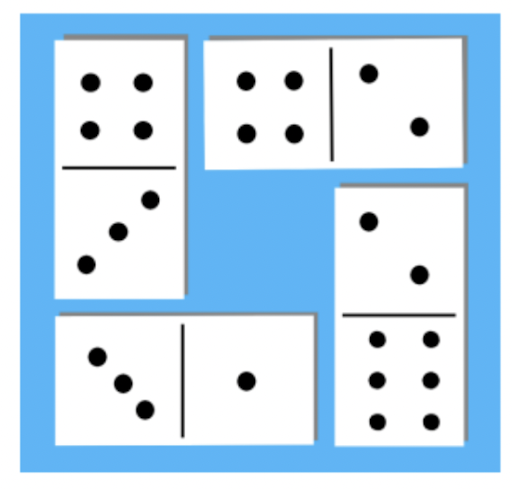
\includegraphics[width=8cm]{text/images/pic3.png}\\
    \caption{Seven Squares}
\end{figure} \newline
După cum se observă și în poză, fiecare 2 capete vecine 3-3 , 4-4 și 2-2, au același număr. Dar, 6!=1.
Se poate găsi o posibilitate pentru a îndeplini toate condițiile?
Vom afla la implementare.

\pagebreak
\subsection{The Resistance - Spy View}

\begin{enumerate}
    \item Prima Problemă\newline\newline
Din punctul de vedere al echipei de spioni, cea mai mare problemă din jocul este încercarea de a afla cine sunt ceilalți spioni. Pentru a avea succes, echipa de spionaj trebuie să lucreze împreună și să-și coordoneze eforturile fără a se lăsa în fața echipei Rezistența.\newline
    \item A doua Problemă\newline\newline
O altă problemă pentru echipa de spionaj este să încerce să saboteze misiunile echipei de Rezistență fără a fi prins. Echipa de spionaj își poate folosi voturile pentru a încerca să blocheze propunerile de misiune, dar dacă sunt prea evidente, echipa Rezistenței poate deveni suspicioasă și poate începe să-și dea seama cine sunt spionii. Aceasta înseamnă că echipa de spionaj trebuie să fie atentă și strategică în modul în care își folosesc voturile și să încerce să saboteze misiunile. \newline

\end{enumerate}

\begin{figure}[h]
    \centering
    
\includegraphics[width=8cm]{text/images/pic4.png}\\
\end{figure} \newline\newline

\newline\newlineÎn general, echipa de spionaj se confruntă cu o serie de provocări în jocul Rezistenței, inclusiv încercarea de a-și da seama cine sunt colegii lor spioni, lucrul împreună fără a se dezvălui și sabotarea eforturilor echipei Rezistență fără a fi prins. Aceste provocări pot face jocul captivant și plin de suspans și necesită ca echipa de spionaj să-și folosească inteligența și gândirea strategică pentru a reuși.

\pagebreak
\section{Implementare}

\textbf{Seven Squares problema 1:}\newline\newline
\textbf{Cod:}\newline\newline

% a se completa fisierul code/ss2.py
\noindent\fbox{%
    \parbox{\textwidth}{%
\inputminted[linenos]{python} {code/ss2.in}\newline\newline
    }%
}
\newline\newline
\newline\newline
 \textbf{Seven Squares problema 2:}\newline\newline
\textbf{Cod:}\newline\newline

% a se completa fisierul code/ss2.py
\noindent\fbox{%
    \parbox{\textwidth}{%
\inputminted[linenos]{python} {code/ss1.in}\newline\newline
    }%
}\pagebreak



\textbf{The Resistance:}\newline\newline
\textbf{Cod:}\newline
% a se completa fisierul code/spy.py
\inputminted[linenos]{python}{code/spy.in}









\include{text/4_Soluții}
\section{Conluzii}
Prover9 și Mace4 pot fi folosite pentru a rezolva diferite tipuri de puzzle-uri și jocuri sociale. În general, acești demonstratori de teoreme funcționează luând un set de ipoteze logice și o formulă de obiectiv ca intrare și apoi încercând să găsească o soluție care să satisfacă ipotezele și obiectivul.\newline\newline
Pentru a utiliza Prover9 și Mace4 pentru puzzle-uri și jocuri sociale, primul pas este să exprimăm regulile și constrângerile puzzle-ului sau jocului ca formule logice.\newline\newline
Odată ce am exprimat regulile și constrângerile puzzle-ului sau jocului ca formule logice, putem folosi Prover9 sau Mace4 pentru a găsi o soluție care să satisfacă aceste formule.
\newline\newline

\begin{figure}[h]
    \centering
    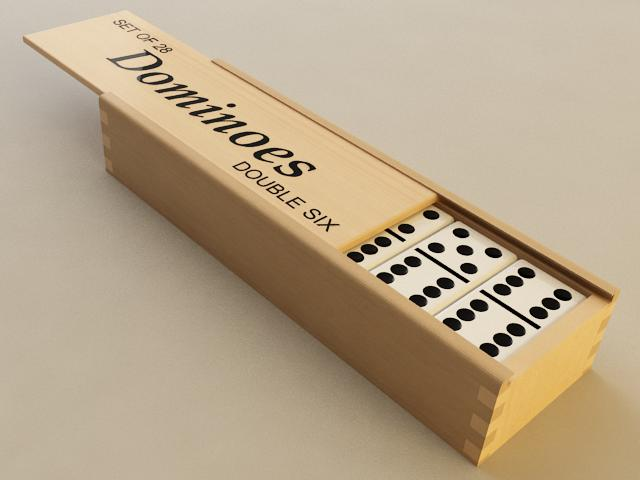
\includegraphics[width5cm]{text/images/pic10.jpg}\\

\end{figure}



\end{document}